\documentclass[11pt,a4paper]{article}

\usepackage[margin=2cm]{geometry}
\usepackage[T1]{fontenc}
\usepackage{lmodern}
\usepackage{graphicx}
\usepackage{booktabs}
\usepackage{hyperref}
\usepackage{booktabs}
\usepackage{graphicx}
\hypersetup{colorlinks=true, urlcolor=blue, linkcolor=black}

\begin{document}

% ---------------------------------------------------------------- cover page
\begin{titlepage}
\centering
\vspace*{2cm}
{\large University of Southern Denmark (SDU)\par}
\vspace{0.5cm}
{\large Embedded Systems (E26)\par}
\vspace{2cm}
{\huge\bfseries Assignment 2\par}
\vspace{0.5cm}
{\Large Accelerated AI for Vision Applications\par}
\vspace{2cm}
\vspace{0.5cm}
Teo Humar\\
Maks Jagodič\\
Mateusz Okula\\
Jérémy Flèche\\
\vspace{2cm}
\textbf{Video:} \url{https://}\par
\vfill
{\large \today\par}
\end{titlepage}

% ---------------------------------------------------------------- report
\section{}

\section{}

\section{}

\section{End-to-end demonstration and comparison}

The complete pipeline PC $\rightarrow$ UART $\rightarrow$ CPU $\rightarrow$ CNN/SNN HLS IP
$\rightarrow$ CPU $\rightarrow$ UART $\rightarrow$ PC was run on the PYNQ-Z2. The PC displays
each input image together with its true label and the class predicted by each network (demo
mode, shown in the video); accuracy is measured on all test images (Fig.~\ref{fig:cm}).

\textbf{Conditions.} Bare-metal ARM application, accelerators at 100\,MHz, the same test
images for both networks (9\,000 images of the shared test split and 12\,000 images of an
additional test set), $60\times60$ 8-bit grayscale images sent as raw pixels over UART at
4\,Mbaud (8N1, 3\,606-byte frame). Inference time is measured on the board with the ARM
global timer from \texttt{ap\_start} to \texttt{ap\_done}; UART time is measured separately.
Resources and power come from the Vivado post-implementation reports.

\begin{table}[h]
\centering
\small
\begin{tabular}{lcc}
\toprule
 & \textbf{CNN} & \textbf{SNN} \\
\midrule
Accuracy, shared test split (9\,000)   & 99.99\,\% & -- \\
Accuracy, additional test set (12\,000) & 99.93\,\% & -- \\
Lowest per-class accuracy               & 99.85\,\% (rectangle) & -- \\
\midrule
Inference latency                       & 1.40\,ms (140\,230 cycles) & -- \\
Accelerator throughput                  & 713\,img/s & -- \\
\midrule
LUT / FF (IP only)                      & 11\,110 / 13\,446 & -- \\
BRAM tiles / DSP (IP only)              & 46.5 / 102 & -- \\
IP dynamic power                        & 0.374\,W & -- \\
Energy per inference (IP)               & 0.52\,mJ & -- \\
\midrule
UART transfer per image                 & 9.01\,ms & -- \\
PC round trip / end-to-end throughput   & 14.7\,ms / 68\,img/s & -- \\
\bottomrule
\end{tabular}
\caption{CNN vs.\ SNN measured on the PYNQ-Z2. Device totals: 22.5\,\% LUT, 33\,\% BRAM,
46\,\% DSP for the CNN build; total on-chip power 1.79\,W, of which 1.26\,W for the ARM.}
\end{table}

\begin{figure}[h]
\centering
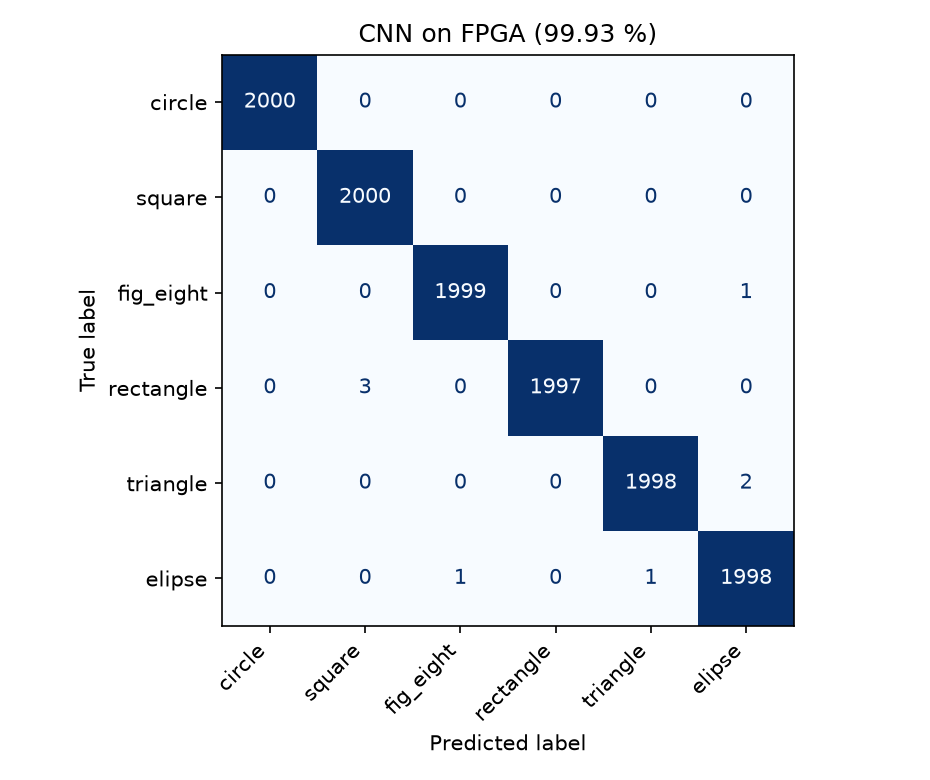
\includegraphics[width=0.48\linewidth]{figures/confusion_cnn.png}\hfill
\includegraphics[width=0.48\linewidth]{figures/confusion_snn.png}
\caption{Confusion matrices on the FPGA (additional test set, 12\,000 images).}
\label{fig:cm}
\end{figure}

\textbf{Communication overhead.} Transferring one image over UART takes 9.01\,ms
(theoretical 9.02\,ms), i.e.\ about 6 times the CNN inference time and 61\,\% of the
14.7\,ms round trip; the rest is mainly USB latency on the PC side. The system is therefore
limited by communication, not by computation: the CNN accelerator alone could process
713\,img/s, the complete system 68\,img/s. A faster link (Ethernet, or sending images in
batches) would be the first improvement.

\end{document}
